\chapter{算法实现与代表方案}

本章介绍已经接入通用协议的具体密码算法，并说明三组代表方案的选择依据。两种HIBE和五种常规
IBS形成十种端到端组合；Wang--PW作为第六种IBS后端，已与LATTE完成一套目标参数组合。各算法
保持独立参数和对象格式，公共协议仅通过第三章定义的接口调用。

\section{分层身份基加密实现}

\subsection{LATTE两层身份委派机制}

LATTE在NTRU结构中实现量子安全HIBE\cite{zhao2024latte}。作品采用LATTE-3参数：多项式次数
$N=1024$、模数$q=68718428161$、分层深度为2。主陷门由短NTRU关系构成，接收身份$r$和发送
身份$s$分别映射为两层身份多项式。发钥机构为$r$生成一级密钥，接收端再为$s$委派叶密钥。

加密端按$(r,s)$生成Ring-LWE型种子密文，叶密钥消去公开环项后恢复32字节随机种子。实现随后进行
确定性重加密核对，排除错误结果落入解码区间的情况。主公钥、主陷门、一级密钥、叶密钥和密文
采用不同对象类型，参数快照与对象一同保存。

实现复用LATTE作者代码中的Gaussian采样和ffSampling路径，并将原生对象封装为严格的Python
后端。每次原生采样后，适配层使用精确环算术检查NTRU关系、委派关系和对象形状。LATTE建立、
一级发钥和在线解密成本较低，因此A、B两组代表都选用该HIBE，使两组主要差别集中在IBS。

\subsection{Lai分层身份块扩展机制}

Lai方案利用理想格陷门完成分层委派\cite{lai2015trapdoors}。根公开向量与短陷门满足
\[
 \mathbf a_0^{\mathsf T}R+\mathbf a_1=\mathbf g.
\]
两层身份分别映射为二进制环元素$\mathrm{id}_1$和$\mathrm{id}_2$，完整身份公开项为
\[
 \mathbf a_{\mathrm{ID}}
 =\mathbf u_0+\mathrm{id}_1\mathbf u_1+\mathrm{id}_2\mathbf u_2.
\]
每委派一层，后端向公开矩阵追加身份块，并为扩展后的矩阵生成新陷门。接收身份对应第一层，认可
发送身份对应第二层。

C组采用$n=2048$、$q=274877976577$、$k=39$、深度2、$p=2$的C2配置。身份映射使用二进制
系数，避免身份乘短矩阵时放大噪声；叶陷门通过Babai反演恢复种子，并检查误差的模$p$结构。该
后端的主要成本是二级委派，因此第五章进一步引入接收会话，使固定身份对只生成一次叶密钥。

\section{身份基签名实现}

\subsection{BNN认证转换与ML-DSA／Falcon接入}

认证转换以普通数字签名为基础构造IBS\cite{galindo2006ibs}。系统建立时，发钥机构生成机构签名
密钥；为身份$s$发钥时，先生成用户普通签名密钥对$(\mathsf{vk}_s,\mathsf{xk}_s)$，再由机构
签署身份与用户验签公钥的规范编码：
\[
 \mathsf{cert}_s=\mathsf{DS.Sign}_{\mathsf{sk}_{\rm CA}}
       (\mathsf{Enc}(s,\mathsf{vk}_s)).
\]
完整IBS签名携带用户公钥、机构证书和用户签名。验证端先检查证书，再检查用户签名。

同一转换核心接入ML-DSA与Falcon。ML-DSA实现采用FIPS~204对象格式\cite{nist2024fips204}；
A组选用ML-DSA-44，其普通公钥为1,312字节、普通签名为2,420字节，转换后的IBS签名为6,237
字节。Falcon后端采用Falcon-512和Falcon-1024的固定作者实现及padded格式\cite{falcon2020}。
两者共享机构证书流程，但底层密钥、签名编码和版本号相互独立。

\subsection{Luo模格身份签名}

Luo后端实现原生模格IBS\cite{luo2024ibs}。身份哈希、消息挑战、响应和提示信息直接进入模格
签名关系，验证者使用主公钥、身份和消息完成验签。后端同时保留参考表示和无损紧凑表示，参考格式与紧凑格式无损互转，并共用签名与验签算法。

Luo分别与LATTE、Lai完成组合。该后端为十种组合提供了独立于SRGG的原生模格IBS路线。

\subsection{SRGG身份目标与消息挑战关系}

SRGG在环$R_Q=\mathbb Z_Q[X]/(X^n+1)$上采用模块格结构。主公钥记为$P$，其中的公开矩阵写为
\[
 A=[I_d\mid\widehat A\mid B].
\]
身份$s$决定目标$h=H_1(P,s)$，用户短见证$y$满足$Ay=h\pmod Q$。令
$\zeta=1+X^{n/2}$，$\zeta^*=1-X^{n/2}$为其环伴随，并令$j=\zeta^*e_1$，其中$e_1$是首个
单位向量。记整数多项式环为$R=\mathbb Z[X]/(X^n+1)$。签名时，$p_0$是根据用户短见证$y$构造的相关扰动向量，维数与响应一致；$c\in\{0,1\}^n$是由$H_2$生成的二元挑战多项式。$u\in R$的系数按方案从中心为$-c/\zeta$相应系数的离散Gaussian中抽取。
签名构造矩阵和响应为
\[
 M_h=[\,2A\mid Qj-2h\,]\pmod{2Q},
 \qquad
 z=p_0+\begin{bmatrix}y\\1\end{bmatrix}(\zeta u+c),
\]
验证者由$W'=M_hz-Qjc$恢复承诺$W'$，重新计算挑战并检查响应范数\cite{jia2025ibs}。扰动与响应保留整数系数，承诺及其恢复在模$2Q$的环中计算。$p_0$引入相关扰动，$y$将身份目标带入响应，$\zeta u+c$绑定本次消息挑战。

B组采用PARAM-I：多项式次数$n=512$、模块秩2、$p=16383$、$Q=15744063$，参数评估中的
量子密钥恢复与伪造成本分别约为95 bit和93 bit。该后端包含大量不同取值范围的整数系数，参考
JSON对象较大。第五章的范围感知编码为公钥、机构状态、用户密钥和签名分别选择位宽，通过无损编码减少对象的保存与传输长度。

\subsection{Sageloli环陷门与非齐次签名方程}

Sageloli的公开向量与主陷门$R$满足
\[
 A=[\bar A\mid g-\bar AR].
\]
为身份$s$发钥时，算法生成身份盐$\rho$并采样身份陷门$T_s$，使
\[
 AT_s=H_1(P,\rho,s)-g\pmod q.
\]
签名另取消息盐$\eta$，通过相关扰动和三进制陪集采样得到响应$z$；验证端检查范数和非齐次模
方程\cite{sageloli2023ibs}。

C组选用PARAM-I：$(d,k,\ell)=(2048,65,132)$、$q=3^{65}$、$r^2=49$。PARAM-II保持同一
算法并增大参数。PARAM-I采样若展开为双精度稠密矩阵，单个矩阵的理论存储约为1.18~TiB。
第五章说明如何利用环结构和逐频率低秩计算完成两档参数的发钥与签名。

\subsection{Wang--PW目标参数矩阵SIS后端}

Wang--PW由Wang基本IBS与Pan--Wagner自适应转换组成，采用矩阵SIS关系，并分别为身份和消息
加入随机盐\cite{wang2024ibme,pan2021ibs}。它在作品中作为IBS后端接入；Wang等人的两层匿名
HIBE与IBS通用构造则规定完整IB-ME协议的组合方式。

目标参数为
\[
 n=512,\qquad q=4294967291,\qquad s_0=4.
\]
令$k=\lceil\log_2q\rceil=32$，gadget宽度$w=nk=16384$，公开矩阵宽度$m=32768$，签名向量
维数$M=49152$。根公开矩阵与陷门满足
\[
 A=[\bar A\mid G-\bar AR].
\]
身份密钥$X$满足$AX+H_1=G\pmod q$，签名短向量$z$满足
\[
 [A,H_1]z=H_2(P,\rho,s,\eta,M')\pmod q.
\]

有限离散Gaussian由独立原生组件执行，Python层负责域分隔哈希、参数快照、规范对象和精确模
方程。公钥约64.0~MiB、机构状态约576~MiB、用户签名
密钥约2.06~GiB、签名约384~KiB。
该实现已完成独立签验、状态恢复以及LATTE组合，实验章单列其服务器资源和分阶段时间。

\section{困难假设、参数档与来源对应}

表~\ref{tab:assumption-source-map}给出报告中实际使用的对应关系。

\begin{longtable}{@{}>{\raggedright\arraybackslash}p{.17\textwidth}>{\raggedright\arraybackslash}p{.15\textwidth}>{\raggedright\arraybackslash}p{.24\textwidth}>{\raggedright\arraybackslash}p{.35\textwidth}@{}}
\caption{实际算法、困难假设与参数来源对应}\label{tab:assumption-source-map}\\
\toprule
\rowcolor{black!8} 算法后端 & 作品职责 & 困难问题与模型 & 采用配置与来源 \\
\midrule
\endfirsthead
\toprule
\rowcolor{black!8} 算法后端 & 作品职责 & 困难问题与模型 & 采用配置与来源 \\
\midrule
\endhead
LATTE-3 & 两层匿名HIBE & NTRU根陷门与RLWE封装；经典ROM & $N=1024$、$q=68718428161$、深度2，采用作者LATTE-3档\cite{zhao2024latte} \\
Lai C2 & 两层HIBE & PLWE（Ring-LWE表示）与理想格陷门 & $n=2048$、$q=274877976577$、$k=39$、深度2，采用C2冻结配置\cite{lai2015trapdoors} \\
BNN／ML-DSA & 认证转换IBS & 认证转换条件；ML-DSA的MLWE／MSIS类模格问题 & BNN身份认证转换与ML-DSA-44，普通签名格式遵循FIPS~204\cite{galindo2006ibs,nist2024fips204} \\
BNN／Falcon & 认证转换IBS & 认证转换条件；Falcon的NTRU格与SIS关系 & BNN身份认证转换与Falcon-512 padded格式\cite{galindo2006ibs,falcon2020} \\
Luo & 原生模格IBS & MLWE用于密钥恢复问题，MSIS用于伪造问题；经典ROM & $N=256$、$(k,\ell)=(11,10)$的作品冻结档\cite{luo2024ibs} \\
SRGG & 原生模格IBS & MLWE／MSIS；QROM & 论文Table~4的PARAM-I：$n=512$、模块秩2、$Q=15744063$\cite{jia2025ibs} \\
Sageloli & 原生环格IBS & RSIS；ROM／QROM & 论文Table~6的结构化PARAM-I：$(d,k,\ell)=(2048,65,132)$\cite{sageloli2023ibs} \\
Wang--PW & 矩阵SIS IBS & SIS；基本构造与自适应转换的随机预言机模型 & 目标档$n=512$、$q=4294967291$、$s_0=4$\cite{wang2024ibme,pan2021ibs} \\
\bottomrule
\end{longtable}
\noindent\begin{minipage}{.98\textwidth}\footnotesize
量子安全工作假设：Wang--PW目标档约115 bit；该配置采用的参数与实现来源见文献及附录材料。
\end{minipage}

\section{已实现算法与组合矩阵}

两种HIBE与五种常规IBS形成表~\ref{tab:implemented-matrix}所示的十种组合。每一格均通过统一
接口完成系统建立、双方发钥、消息加密、匹配解密和身份错配拒绝。组合按底层HIBE与IBS算法配对统计。

\begin{table}[H]
\centering\small
\caption{两种HIBE与五种常规IBS的端到端组合}
\label{tab:implemented-matrix}
\begin{tabular}{@{}lccccc@{}}
\toprule
\rowcolor{black!8} HIBE & BNN＋ML-DSA & BNN＋Falcon & Luo & SRGG & Sageloli \\
\midrule
LATTE & 完成 & 完成 & 完成 & 完成 & 完成 \\
Lai & 完成 & 完成 & 完成 & 完成 & 完成 \\
\bottomrule
\end{tabular}
\end{table}

Wang--PW在常规矩阵之外完成LATTE＋Wang--PW端到端组合。当前已实现范围因此包括十种常规
组合和这一套目标参数组合。

\section{代表方案的性能指标与选取依据}

十种常规组合用于检验通用接口并比较成本分布，A、B、C三组分别覆盖低延迟标准化签名路径、具有
紧凑编码的原生模格IBS，以及采用另一种HIBE与环格IBS的连续通信路径。LATTE＋Falcon
与A具有相近的在线时间和更短的密文，但二者同属BNN认证转换路线，因此保留ML-DSA作为主演示。表~\ref{tab:representatives}列出三组算法和容量。

\begin{table}[H]
\centering\small
\caption{三组代表的算法构成与应用消息容量}
\label{tab:representatives}
\begin{tabularx}{\textwidth}{@{}cp{.16\textwidth}Xp{.18\textwidth}@{}}
\toprule
\rowcolor{black!8} 组 & HIBE & IBS & 应用消息上限 \\
\midrule
A & LATTE-3 & BNN／ML-DSA-44 & 59,191 B \\
B & LATTE-3 & SRGG PARAM-I紧凑格式 & 65,364 B \\
C & Lai C2 & Sageloli PARAM-I & 3,924 B \\
\bottomrule
\end{tabularx}

\end{table}

表~\ref{tab:representative-indicators}从第七章的Ultra~9~275HX十组同机基本比较中摘出三组代表。
三组使用相同源码、运行时、线程配置、64字节双方身份和32字节消息；每种组合建立一套独立系统
及主密钥（下称“独立根”），表中各项均为一次实测值。

\begin{table}[H]
\centering\small
\caption{三组代表的主要性能与资源指标}
\label{tab:representative-indicators}
\begin{tabularx}{\textwidth}{@{}>{\raggedright\arraybackslash}p{.27\textwidth}>{\raggedright\arraybackslash}X>{\raggedright\arraybackslash}X>{\raggedright\arraybackslash}X@{}}
\toprule
\rowcolor{black!8} 指标 & A & B & C \\
\midrule
% BEGIN DATA ten-representatives.tex
首次加密 & 12.9~ms & 17.6~s & 96.4~s \\
首次解密 & 103~ms & 125~ms & 412~s \\
重复加密 & 13.5~ms & 11.3~s & 89.4~s \\
重复解密 & 59.4~ms & 68.7~ms & 409~s \\
恢复后解密 & 61.6~ms & 68.2~ms & 406~s \\
完整密文 & 139~KiB & 146~KiB & 4.34~MiB \\
% END DATA ten-representatives.tex
\bottomrule
\end{tabularx}
\begin{minipage}{.96\textwidth}\footnotesize
“重复”表示同一进程、同一套已生成对象下的第二次操作；“恢复后解密”表示新进程加载规范对象后
完成的解密。表中C组执行完整委派路径；会话路径的阶段数据在第五章和第七章单独列出。
\end{minipage}
\end{table}

\begin{figure}[H]
\centering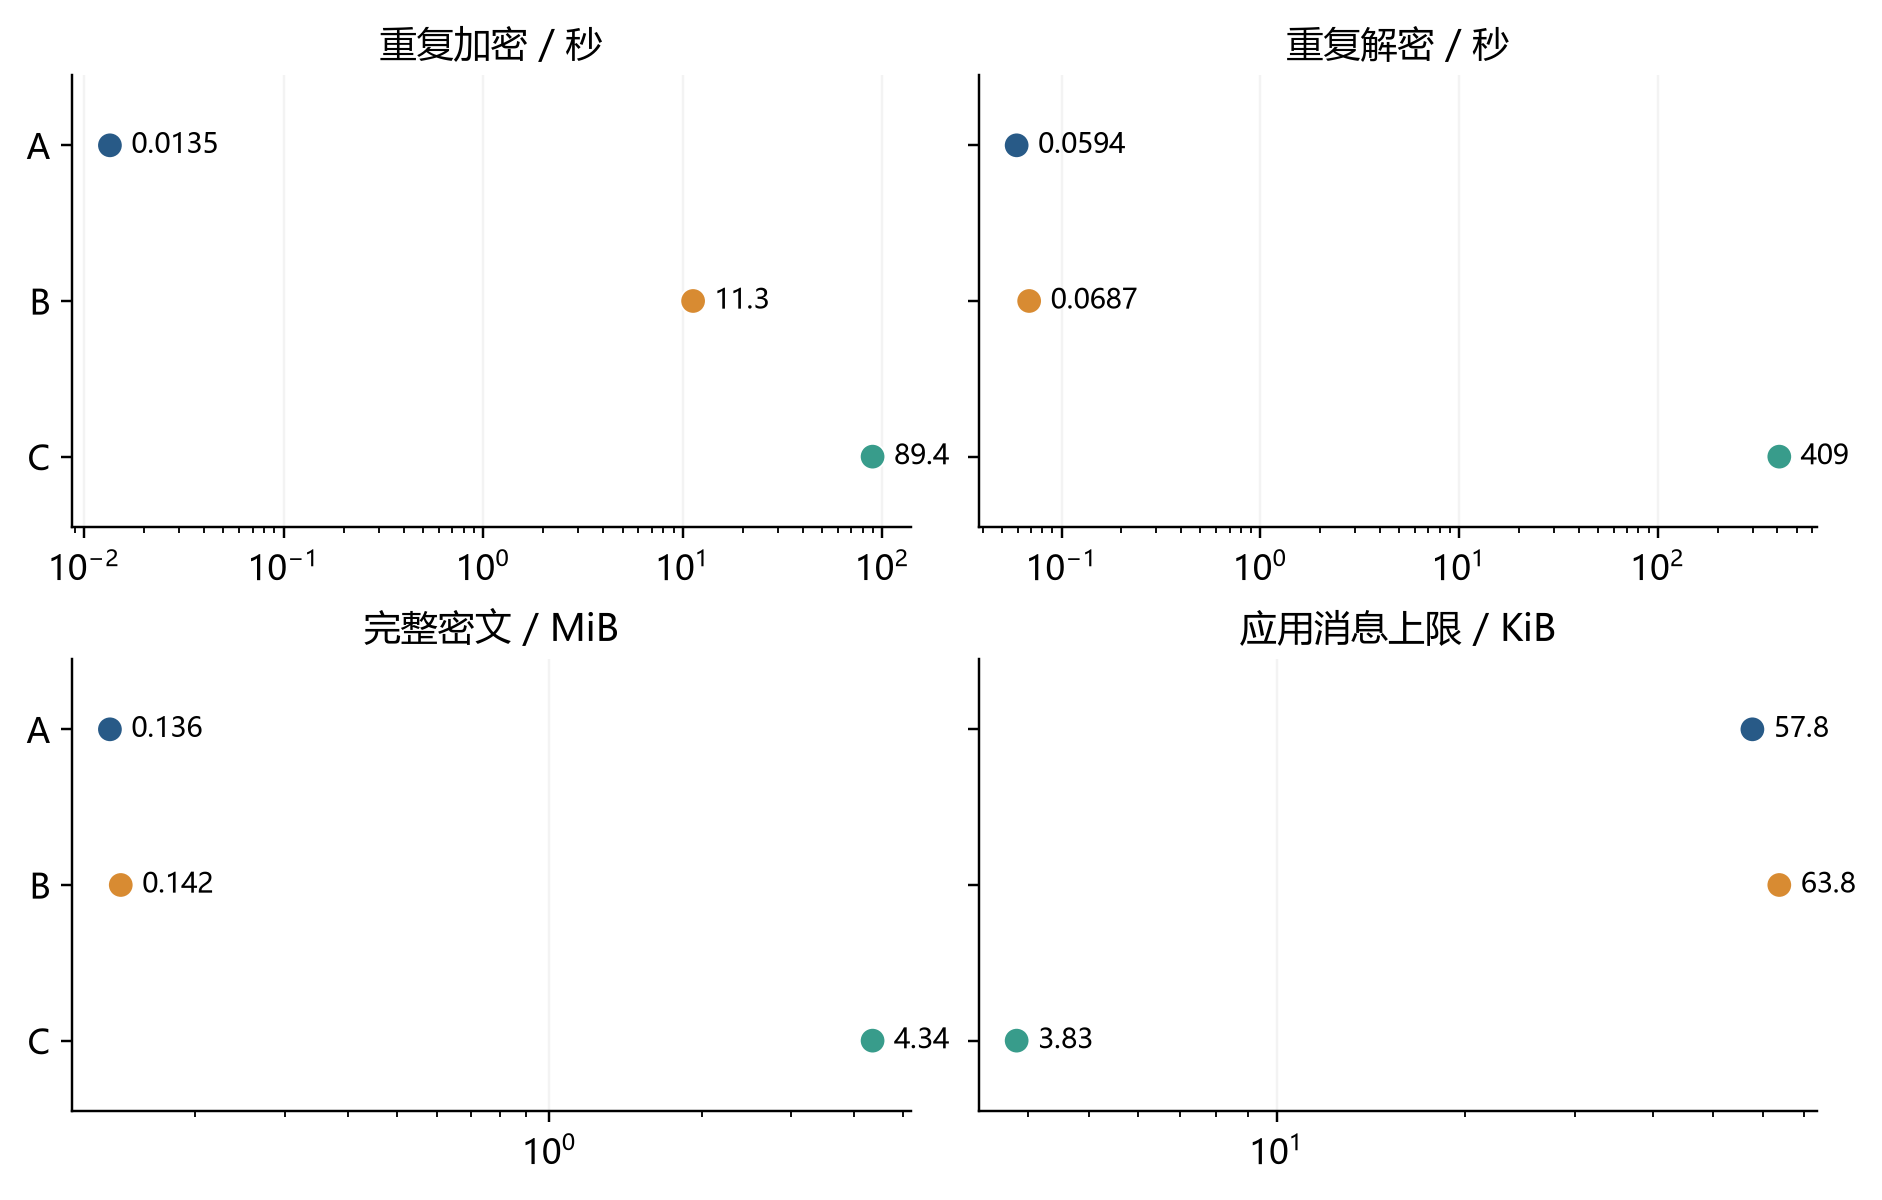
\includegraphics[width=.96\textwidth]{figures/representative-profile.png}
\caption{三组代表方案的同机时间、完整密文与应用容量；各面板使用原始量和对数刻度}
\label{fig:representative-profile}
\end{figure}

同机结果使三组差异可以直接落到协议阶段。A的首次和重复收发均处于亚秒级；B的接收时间与A
接近，主要增加发送方密钥生成和加密中的SRGG签名成本；C的加密、解密和密文长度均明显增加，重点
在于验证Lai与Sageloli能够进入同一完整协议，并为第五章的会话与结构化采样优化提供对象。
十种组合的完整时间、对象尺寸和内存对照见第七章。

\section{三组代表的应用定位}

\subsection{A组：低延迟定向消息}

A组采用LATTE-3与BNN／ML-DSA-44。其重复加密和解密均处于亚秒级，适合需要交互响应的机构
消息、浏览器演示和频繁的小消息收发。ML-DSA组件具有固定标准对象格式，认证转换也便于复用
普通签名实现。A组的主要通信开销来自一次性认证，因此后续优化重点是外层认证
结构和整包长度。

\subsection{B组：原生模格身份认证与紧凑状态}

B组采用LATTE-3与SRGG PARAM-I。其接收端时间与A接近，主要额外成本集中在发送方密钥生成和
签名。范围感知编码显著减少SRGG机构状态、用户密钥和签名长度。该组适合发送端能够承担十余秒签名、
接收端需要快速验证的批量定向投递，也适合研究原生模格IBS和紧凑对象在完整协议中的作用。

\subsection{C组：固定身份对的连续通信}

C组采用Lai C2与Sageloli PARAM-I。初次解密需要完成高成本叶密钥委派，密文也明显大于A、B；
建立接收会话后，同一身份对的后续解密不再重复委派。因而，C组更适合双方身份固定、允许离线
准备并连续处理多条消息的使用方式，例如固定管理端与受控终端之间的周期消息。该组还展示了
高成本HIBE与环格IBS如何通过结构化采样和会话复用进入完整系统。

\section{本章小结}

本章说明了两种HIBE与六种IBS的算法关系和实现对象，并区分十种常规组合与LATTE＋Wang--PW
目标参数组合。A、B、C三组分别代表低延迟认证转换、原生模格身份签名和固定身份对的高成本
环格路线。三组的差异同时体现在在线时间、对象尺寸和可复用的准备状态。
